\chapter{High-pass and low-pass filters}
The main purpose of filters is to remove unwanted frequencies from different signals. Filters are often used on sound files, to control the bass or the high pitch noises. There are different kinds of filters that can remove unwanted frequencies. This section focuses on high and low-pass filters.
\section{Definitions}
In this section the most central terms concerning high-pass and low-pass filters will be defined. The definitions are essential when understanding the most important derivations in the next section \ref{Derivations}.
\subsection{Low-pass filters}
A low-pass filter passes frequencies from  $0~Hz$ to a certain cut-off frequency, after which the amplitude of the signal is decreased.  
\\
In the illustration below the voltage output is measured across the capacitor, which decreases the high frequencies and leaves the low frequencies unchanged.
\\
\begin{figure}[H]
	\begin{center}
\begin{circuitikz}[american voltages]
\draw (0,0)
to[sqV, sqV=$V_{AC}$] (0,2)
to (6,2)
to[short, -] (4,2)
to[C=$C$] (4,0)
to (6,0)
to (4,0)
to [resistor, R=$R$] (0,0);
\draw [>=latex', <->] (6,1.75) -- node[anchor=west] {$V_{output}$} (6,0.25);
\end{circuitikz}
\end{center}

	\caption{Circuit diagram of a low-pass filter.} \label{lp:diagram}
\end{figure} 
\subsection{High-pass filters}
High-pass filters are in many ways similar to the low-pass filters. High-pass filters cuts off frequencies below a certain cut-off frequency. \\
The voltage output is measured across the resistor ($R$) instead of the capacitor ($C$). 
\begin{figure}[H]
	\begin{center}
\begin{circuitikz}[american voltages]
\draw (0,0)
to[sV, sV=$V_{AC}$] (0,2)
to (6,2)
to[short, -] (4,2)
to[resistor, R=$R$] (4,0)
to (6,0)
to (4,0)
to [C=$C$] (0,0);
\draw [>=latex', <->] (6,1.75) -- node[anchor=west] {$V_{output}$} (6,0.25);
\end{circuitikz}
\end{center}

	\caption{Circuit diagram of a high-pass filter.}
	\label{hp:diagram}
\end{figure} 

\subsection{Bode Plots}
Bode plots are two separate graphical representations of the magnitude response (also called the gain) and phase response of a system (versus/) with respect to frequency. They are especially useful in analysing frequency-dependent systems and networks such as filters, tuners, and amplifiers. \cite [p. 626]{bcircuit5}  \\
\\
The magnitude response is plotted in a coordinate system with a logarithmic $x$-axis. For a low-pass filter, the output wave before the cut-off point will remain almost unchanged. After the cut-off point, the output decreases by $20 dB$ per decade, the amplitude decreases and approaches a graph similar to that of DC current. \\
The Bode magnitude plot for a high-pass filter starts in minus decibel and approaches zero. Until it reaches the cut-off point, the graph increases with $20 dB$ per decade. When reaching the cut-off point, the graph is $3 dB$ less than the input signal. Furthermore, $70.7\% (100\%-29.3\%)$ of the amplitude is cut off at the point $f_{cutoff}$.

\subsection{Cut-off Frequencies}
The cut-off frequency for a low-pass filter is the frequency at which the bode plot is decreased by $3dB$, and for a high-pass filter it is when the bode plot is $3dB$ away from reaching zero. The cut-off frequency is also the frequency, where the filtering (both high- and low-pass filters) starts getting efficient. The definition of a cut-off frequency is when the effect in watts is halved. The amount of decibel can be calculated as follows: \cite[p. 596-597]{bcircuit}
\begin{align} \label{number:db}
Number \ of \ dB = 10 \log \left(\dfrac{P_{output}}{P_{input}} \right)
\end{align}
If the halved effect is inserted the $3dB$ can be found:
\begin{align*} 
10 \log \left(\dfrac{1}{2} \right) = -3 dB
\end{align*}
From section \ref{}, the effect, $P$, is defined as $P=\dfrac{v^2}{R}$:
\begin{align*}
Number \ of \ dB = 10 \log \left(\dfrac{\dfrac{v_{output}^2}{R}}{\dfrac{v_{input}^2}{R}} \right)
\end{align*}
This can be simplified:
\begin{align} \label{number:db:volt}
Number \ of \ dB = 10 \log \left(\left(\dfrac{v_{output}}{v_{input}} \right)^2\right)
\end{align}
From equation \eqref{number:db} and \eqref{number:db:volt} the following relation can be derived: $$\dfrac{P_{output}}{P_{input}}= \left(\dfrac{v_{output}}{v_{input}} \right)^2$$ To find the point at which the power is halved, the right side of the above equation can be set equal to $\dfrac{1}{2}$:
\begin{align*}
\dfrac{1}{2}= \left(\dfrac{v_{output}}{v_{input}} \right)^2
\end{align*}
This can be simplified:
\begin{align} \label{vratio:equal}
\dfrac{1}{\sqrt{2}}= \dfrac{v_{output}}{v_{input}}
\end{align}
From equation \eqref{vratio:equal} it can be found that the amplitude is decreased by $1-\left(\dfrac{1}{\sqrt{2}} \right) = 29.3\%$.

\subsection{The imaginary Angular Frequency}
The experiment in chapter \ref{chap:RC} for testing the capacitor used a DC voltage. In the case of high and low pass filters, an AC input will be applied. The voltage, in this case, can be written as a wave function:
\begin{align}
v(t)=A\sin(\omega_f t+\theta)
\end{align}
Where $A$ is the amplitude, $\omega_f=2\pi f$ and $\theta$ the phase shift. In this section, it is considered that there is no phase shift on the input sinus wave. According to definition \ref{lpdef}, $s=\sigma + i \omega$. Here $i \omega$ can be considered the imaginary angular frequency, if the real part is set to zero $\sigma = 0$. Hereby $s$ can be rewritten as $s = i \omega_f$ \cite[p. 733 - 735]{bcircuit9}.

\section{Derivations} \label{Derivations}
Intro bliver skrevet.
\subsection{Transfer Function for Low-Pass Filters}
From the transient analysis, equation \eqref{eq:dvC(t)} is derived:
\begin{align} \label{eq:dV_C}
\dfrac{dv_C(t)}{dt}=-v_R(t)\dfrac{1}{RC}
\end{align}
From KVL the algebraic sum of voltages can be written as: 
\begin{align}
v_{input}(t)-v_{R}(t)+v_{C}(t)=0
\\
\Leftrightarrow -v_{R}(t) = v_{input}(t) - v_{C}(t) \label{eq:KVL_low}
\end{align}
\eqref{eq:KVL_low} is inserted in \eqref{eq:dV_C}:
\begin{align} 
\dfrac{dv_C(t)}{dt}&=\Big(v_{input}(t) - v_{C}(t)\Big)\dfrac{1}{RC}
\\
&=\dfrac{1}{RC}v_{input}(t) - \dfrac{1}{RC}v_{C}(t)
\end{align}
Both sides are added with $\dfrac{1}{RC}v_C(t)$:
\begin{align}
\dfrac{dv_C(t)}{dt}+\dfrac{1}{RC}v_C(t)=\dfrac{1}{RC}v_{input}(t)
\end{align}
The differential equation can now be solved using the Laplace transform:
\begin{align}\label{eq:laplace:low}\mathcal{L}\bigg\{\dfrac{dv_C(t)}{dt}\bigg\}+\dfrac{1}{RC}\mathcal{L}\Big\{v_C(t)\Big\}=\dfrac{1}{RC}\mathcal{L}\Big\{v_{input}(t)\Big\}
\end{align}
According to \Cref{theorem:lap_diff}, the Laplace transform of \eqref{eq:laplace:low} yields the following equation:
\begin{align}
V_C(s)s+v_C(0)+\dfrac{1}{RC}V_C(s)=\dfrac{1}{RC}V_{input}(t)
\end{align} 
$v_{C}$ is now factorised, and the initial voltage across the capacitor is zero, which can be derived from equation \eqref{V_up}:
\begin{align}
\dfrac{1}{RC}V_{input}(s)=V_{C}(s)\Big(\dfrac{1}{RC}+s\Big)
\end{align} 
The ratio of the voltages is isolated:
\begin{align}
\dfrac{\dfrac{1}{RC}}{\dfrac{1}{RC}+s} = \dfrac{V_{C}(s)}{V_{input}(s)}
\end{align} 
As stated in REF(hjælp afsnit 7.1.6), $s=i \omega_f$. Furthermore, the expression $\dfrac{V_{C}(s)}{V_{input}(s)}$ is defined as the transfer function for low-pass filters, $H_{L}(s)$. Since $s$ is redefined the $H_{L}(s)=H_{L}(i \omega_f)$:
\begin{align} \label{eq:trans_low}
H_{L}(i \omega_f) = \dfrac{\dfrac{1}{RC}}{\dfrac{1}{RC}+i \omega_f} 
\end{align}
Both sides of the equation is multiplied by $\dfrac{RC}{RC}$:
\begin{align}
H_{L}(i \omega_f) = \dfrac{RC}{RC} \cdot \dfrac{\dfrac{1}{RC}}{\dfrac{1}{RC}+i \omega_f} 
\end{align}
This can be simplified:
\begin{align}
H_{L}(i \omega_f) =  \dfrac{1}{1+RC \cdot i \omega_f} 
\end{align}
Now the length of the both sides is calculated as in \eqref{eq:mod_div}:
\begin{align}
\left|H_{L}(i \omega_f) \right| &=  \left|\dfrac{1}{1+RC \omega_f} \right| 
\\
&=\dfrac{|1|}{|1+RC\omega_f |}
\\
&=  \dfrac{1}{\sqrt{1+(RC \omega_f)^2}} \label{tf:mod}
\end{align}
Equation \eqref{tf:mod} describes the numerical relationship between the input and the output signal.
\subsection{Transfer Function for High-Pass Filters}
Similarly, to the low pass filter, the transfer function is derived from equation \eqref{eq:dvC(t)} 
\begin{align}
\dfrac{dv_{c}(t)}{dt} = -v_{R}(t) \cdot \dfrac{1}{RC}
\end{align}
First both sides are multiplied by $-RC$:
\begin{align}
-RC \cdot \dfrac{dv_{c}(t)}{dt} = v_{R}(t)
\end{align}
Since it is now a high-pass filter (and a different circuit), KVL has to be rewritten and is now $v_{C}(t)=v_{R}(t)-v_{input}(t)$. Both sides of this expression are now differentiated, and can be inserted on the left side as follows:
\begin{align*}
-RC \cdot \left(\dfrac{dv_{R}(t)}{dt} - \dfrac{dv_{input}(t)}{dt} \right) = v_{R}(t)
\end{align*}
The Laplace transform is now applied to both sides of the equation. Note that $RC$ is a constant and can be moved outside the transform per definition \ref{constant}:
\begin{align*}
-RC \mathcal{L} \left\{\dfrac{dv_{R}(t)}{dt} \right\} + RC \mathcal{L} \left\{ \dfrac{dv_{input}(t)}{dt} \right\} = \mathcal{L} \left\{v_{R}(t) \right\}
\end{align*}
The values can be found from the table \ref{lptable} in the previous chapter:
\begin{align*}
-RCsV_{R}(s)-v_{R}(0) + RCsV_{input}(s)-v_{input}(0) = V_{R}(s)
\end{align*}
It is assumed that the phase shift is zero and $v_{R}(0)$ and $v_{input}(0)$ are both equal to zero:
\begin{align*}
-RCsV_{R}(s) + RCsV_{input}(s) = V_{R}(s)
\end{align*}
Now $RCs V_{input}(s)$ is isolated:
\begin{align*}
RCsV_{input}(s) = V_{R}(s) + RCsV_{R}(s)
\end{align*}
$V_{R}(s)$ is factorised:
\begin{align*}
RCsV_{input}(s) = V_{R}(s) \cdot (1 + RCs)
\end{align*}
The ratio of the voltages is isolated:
\begin{align} \label{hp:visolated}
\dfrac{RCs}{1 + RCs} = \dfrac{V_{R}(s)}{V_{input}(s)}
\end{align}
The expression $\dfrac{V_{R}(s)}{V_{input}(s)}$ can be described as the transfer function of high-pass filters, $H_{H}(s)$. As stated in REF(hjælp afsnit 7.1.6) then $s=i \omega_f$. Therefore $H_{H}(s)=H_{H}(i \omega_f)$. The equation \eqref{hp:visolated} can be rewritten:
\begin{align*}
H_{H}(i \omega_f) = \dfrac{RCi \omega_f}{1 + RCi \omega_f}
\end{align*}
The length of both sides can be calculated. When taking the modulus of a complex number, the following rule from definition \ref{modulus} is used: $|z|= \sqrt{a^2+b^2}$. The expression is calculated as follows:
\begin{align}
\left|H_{H}(i \omega_f)\right| &= \left|\dfrac{RCi \omega_f}{1 + RCi \omega_f} \right| \\
 &= \dfrac{|RCi \omega_f|}{|1 + RCi \omega_f |} \\
 &= \dfrac{\sqrt{(RC \omega_f)^2}}{\sqrt{1 + (RC \omega_f)^2 }} \\
 &= \dfrac{RC \omega_f}{\sqrt{1 + (RC \omega_f)^2 }} \label{tfmodhp}
\end{align} 
Equation \eqref{tfmodhp} describes the numerical relationship between the input and output signal.
\subsection{Cut-Off Frequency}
The right side of the equation \eqref{vratio:equal} can be set equal to the transfer function \ref{eq:trans_low}. The cut-off frequency can be found from the transfer function for either high-pass or low-pass filters. In this case the function for low-pass filter is used.
\\
\begin{align*}
\dfrac{1}{\sqrt{1+ \left(RC \cdot \omega_f \right)^2}} = \dfrac{1}{\sqrt{2}}
\end{align*}
To get rid off the square root, both sides are squared:
\begin{align*}
\dfrac{1}{1+ \left(RC \cdot \omega_f \right)^2} = \dfrac{1}{2}
\end{align*}
	Both sides are multiplied by $2(1+(RC\omega_f)^2)$:
\begin{align*}
2 = 1+ \left(RC \cdot \omega_f \right)^2
\end{align*}
Both sides are subtracted by 1, and then raised to the power of $\dfrac{1}{2}$:
\begin{align*}
1 = RC \cdot \omega_f 
\end{align*}
Note that from equation \eqref{eq:omega}, $\omega_f$ is defined as $\omega_f=2 \pi f$:
\begin{align*}
1 = RC 2\pi f 
\end{align*}
Now $f$ is isolated:
\begin{align*}
f=\dfrac{1}{2\pi RC}
\end{align*}
Hereby the cut-off frequency is derived. It can now be shown that the cut-off frequency is after 3 decibel, by inserting the initial values on equation \eqref{number:db}:
\begin{align*}
10 \log \left(\dfrac{1}{2} \right) = -3 dB
\end{align*}
\section{Experiment} \label{experiment}
- Her kommer der en beskrivelse af eksperimentet
\subsection{Theoretical}
The expected values of the bode plot, were computed using the following formulas:
\begin{align}
	V_{out} =& V_{in} \cdot \dfrac{X_C}{\sqrt{R^2+X_{C}^2}},
\end{align}
in the case of low-pass filters and:
\begin{align}
	V_{out} =& V_{in} \cdot \dfrac{R}{\sqrt{R^2+X_{C}^2}},
\end{align}
in the case of high-pass filters.
Where $R$ is the resistance of the resistor (in ohms, $\Omega$), $V_{in}$ is the input voltage (in volts, $V$), and $V_{out}$ is the output voltage (in volts, $V$).
\\
In the formulas $X_C$ is the capacitive reactence for the capacitor. This value is calculated as follows:
\begin{align*}
	X_C =& \dfrac{1}{2\pi fC}
\end{align*}
In this case $f$ is the frequency of the input signal (in hertz, $Hz$), and $C$ is the capacitance of the capacitor (in farad, $F$). $X_C$ is then the resistance across the capacitor, as a function of frequency and capacitance.
\\
\\
The gain of the signal going through the circuit, which is plotted on the y-axis, is defined as:
\begin{align*}
	gain = 20 \cdot \log{\left( \dfrac{V_{out}}{V_{in}} \right)}
\end{align*}
\\
\\
To find the expected gain of the signal, the resistance and capacitance of the circuit were defined in Python. A function which calculates the gain, as a function of frequency, was defined. This function took an array of frequencies as its argument.
\\
The input and output of the Python function was then plotted.
\subsection{Test Values}
- How did we get the results we did? What circuit --> refer to description after intro \\
Low-pass: \\
The bode plot looks like this:
\begin{figure}[H]
\center
	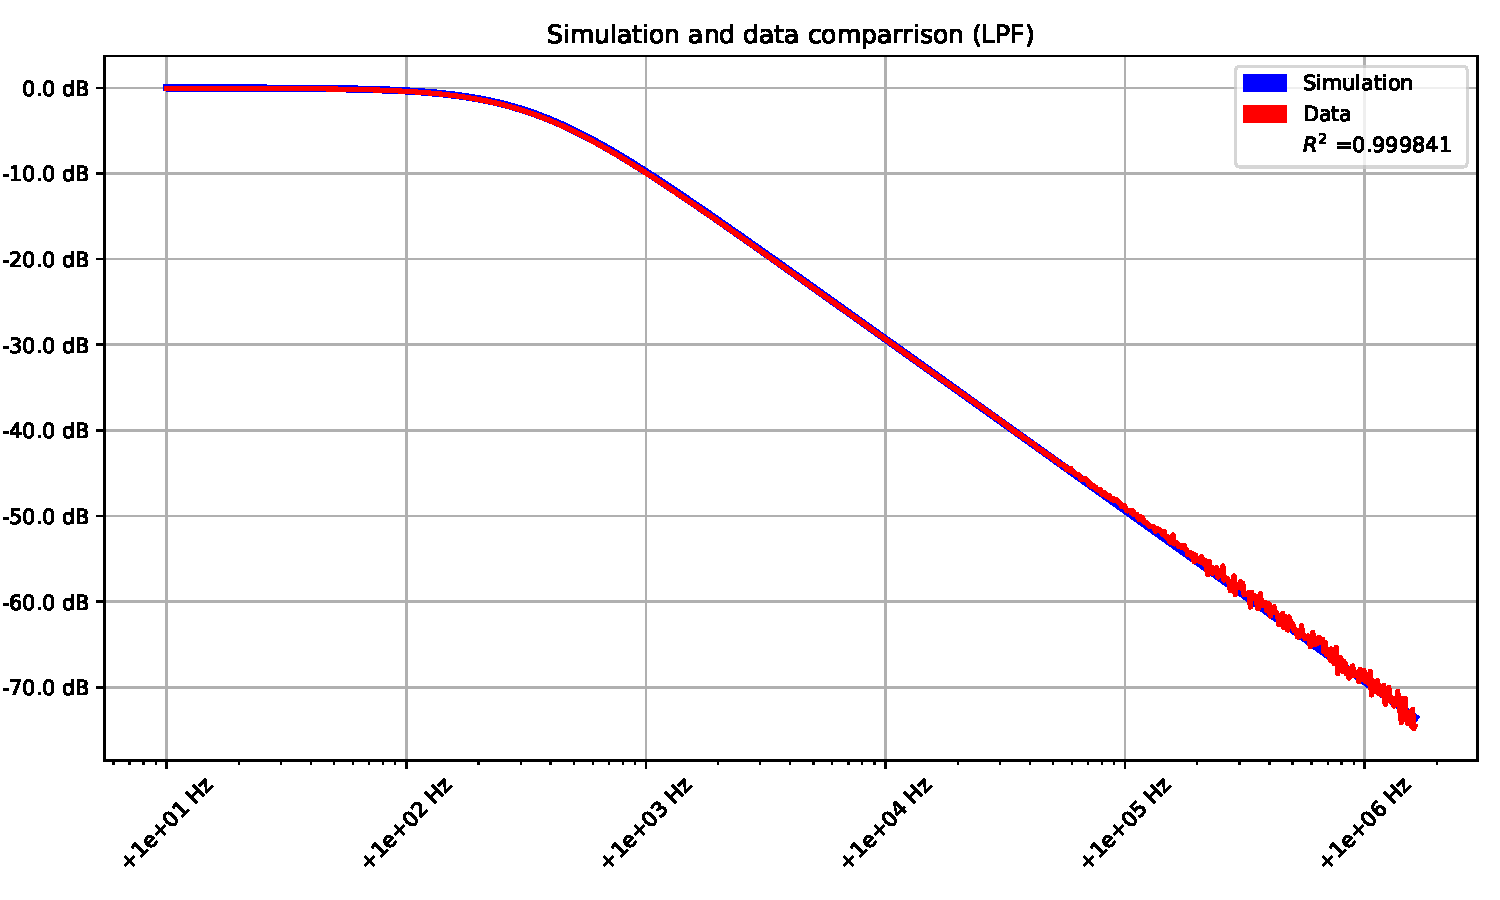
\includegraphics[scale=0.5]{fig/img/bode_LPF_plot.pdf}
	\caption{Low-pass bode plot}
	\label{lp:bode}
\end{figure}
High-pass: \\
Here is the bode plot:
\begin{figure}[H]
\center
	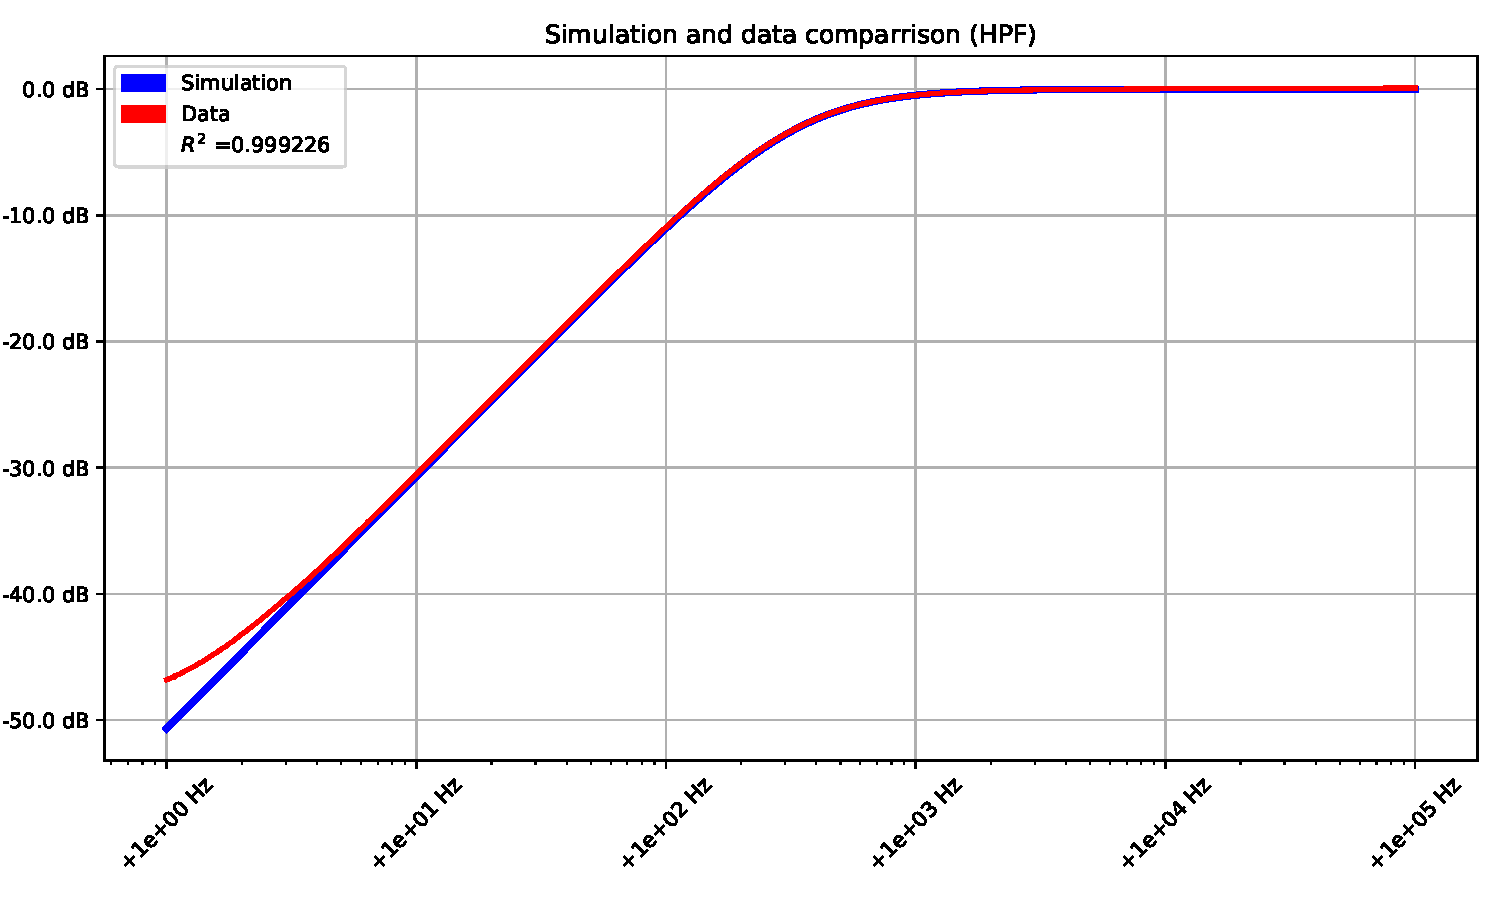
\includegraphics[scale=0.5]{fig/img/bode_HPF_plot.pdf}
	\caption{High-pass bode plot}
	\label{hp:bode}
\end{figure}
\subsection{Comparison}
- Compare the bode plots --> first low then high \\
- Describe source errors (fejlkilder)
